\begin{frame}[plain]
  \begin{figure}
    \centering
    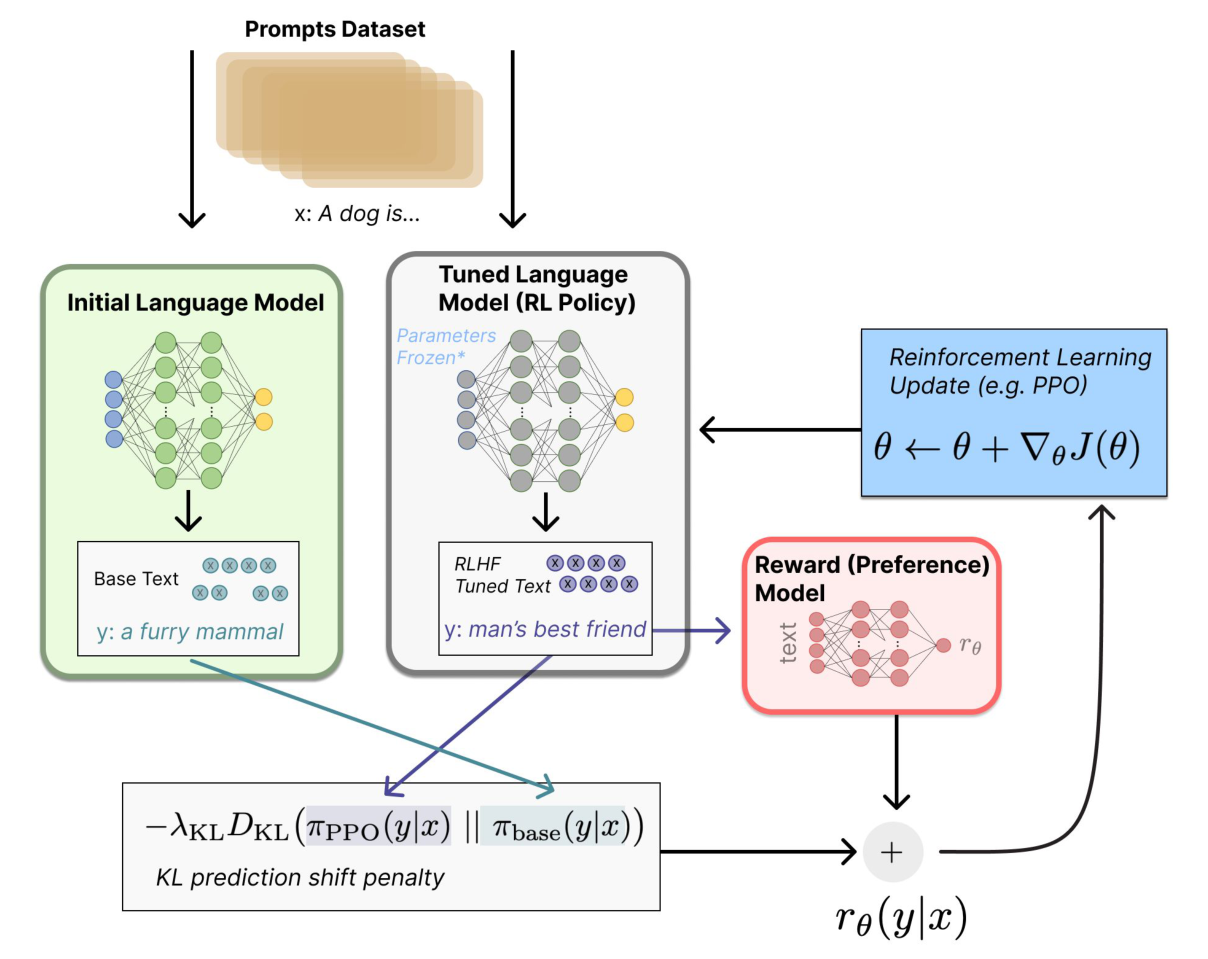
\includegraphics[width=0.8\paperwidth,height=0.72\paperheight,keepaspectratio]{images/llm-rlhf/rlhf_ppo_overview_pipeline.png}
    \caption*{\scriptsize Lambert, Castricato, von Werra \& Havrilla, ``Illustrating Reinforcement Learning from Human Feedback (RLHF),'' Hugging Face Blog, 2022.}
  \end{figure}
\end{frame}

\begin{frame}[t]{Table of Contents}
  \scriptsize
  \begin{enumerate}
    \item \textcolor{red}{Motivation}
    \item Learning Outcomes
    \item \textcolor{red}{Fine-Tuning Methods for LLMs}
    \begin{enumerate}
      \scriptsize
      \item Categories of Fine-Tuning
      \item \textcolor{red}{Full Fine-Tuning (FT)}
      \item \textcolor{red}{Parameter-Efficient Fine-Tuning (PEFT)}
    \end{enumerate}
    \item \textcolor{red}{Supervised Fine-Tuning (SFT)}
    \begin{enumerate}
      \scriptsize
      \item What is SFT?
      \item Datasets for SFT
      \item Domain-Specific SFT
      \item Limitations of SFT
    \end{enumerate}
    \item \textcolor{red}{RLHF --- Reinforcement Learning with Human Feedback}
    \begin{enumerate}
      \scriptsize
      \item Why RLHF?
      \item The RLHF Pipeline
    \end{enumerate}
  \end{enumerate}
\end{frame}

\begin{frame}[t]{Table of Contents (cont.)}
  \scriptsize
  \begin{enumerate}
    \setcounter{enumi}{5}
    \item \textcolor{red}{Reward Model (RM)}
    \item \textcolor{red}{RLHF Training with PPO}
    \item \textcolor{red}{Direct Preference Optimization (DPO)}
    \item \textcolor{red}{Beyond DPO: ORPO and KTO}
      \begin{enumerate}
        \scriptsize
        \item ORPO
        \item KTO
      \end{enumerate}
    \item \textcolor{red}{Constitutional AI and RLAIF}
      \begin{enumerate}
        \scriptsize
        \item Constitutional AI
        \item RLAIF
      \end{enumerate}
    \item \textcolor{red}{LoRA and Quantized LoRA}
      \begin{enumerate}
        \scriptsize
        \item What is LoRA?
        \item Benefits of LoRA
        \item What is QLoRA?
        \item Applications of LoRA / QLoRA
      \end{enumerate}
  \end{enumerate}
\end{frame}

\begin{frame}[t]{Table of Contents (cont.)}
  \scriptsize
  \begin{enumerate}
    \setcounter{enumi}{11}
    \item \textcolor{red}{PEFT Beyond LoRA}
      \begin{enumerate}
        \scriptsize
        \item Prefix and Prompt Tuning
        \item Adapters and (IA)$^3$
        \item DoRA
        \item Choosing a PEFT Method
      \end{enumerate}
    \item \textcolor{red}{Model Merging and Continual Learning}
      \begin{enumerate}
        \scriptsize
        \item Task Vectors and Task Arithmetic
        \item Merging Recipes
        \item Continual Learning and Forgetting
      \end{enumerate}
    \item \textcolor{red}{Limitations of Fine-Tuning and RLHF}
    \item \textcolor{red}{Future Directions}
    \item \textcolor{red}{Summary}
  \end{enumerate}
\end{frame}
